%%%%%%%%%%%%%%%%%%%%%%%%%%%%%%%%%%%%%%
% LaTeX poster template
% Created by Nathaniel Johnston
% August 2009
% http://www.nathanieljohnston.com/2009/08/latex-poster-template/
%%%%%%%%%%%%%%%%%%%%%%%%%%%%%%%%%%%%%%

\documentclass[handout,final]{beamer}
\usepackage{beamerposter}
\usepackage{graphicx}			% allows us to import images

\usepackage{bm}
\usepackage{tikz}

\usetikzlibrary{trees,shadows}

\tikzset{/tikz/x=2.5cm}
\tikzset{/tikz/y=2.5cm}

%-----------------------------------------------------------
% Define the column width and poster size
% To set effective sepwid, onecolwid and twocolwid values, first choose how many columns you want and how much separation you want between columns
% The separation I chose is 0.024 and I want 4 columns
% Then set onecolwid to be (1-(4+1)*0.024)/4 = 0.22
% Set twocolwid to be 2*onecolwid + sepwid = 0.464
%-----------------------------------------------------------

\newlength{\sepwid}
\newlength{\onecolwid}
\newlength{\twocolwid}
\newlength{\threecolwid}
\setlength{\paperwidth}{48in}
\setlength{\paperheight}{36in}
\setlength{\sepwid}{0.024\paperwidth}
\setlength{\onecolwid}{0.22\paperwidth}
\setlength{\twocolwid}{0.464\paperwidth}
\setlength{\threecolwid}{0.708\paperwidth}
\setlength{\topmargin}{-0.5in}
\usetheme{confposter}
\usepackage{exscale}

% New math commands/abreviations

\newcommand{\bA}{\mathbf{A}}
\newcommand{\bB}{\mathbf{B}}
\newcommand{\bC}{\mathbf{C}}
\newcommand{\bD}{\mathbf{D}}
\newcommand{\bE}{\mathbf{E}}
\newcommand{\bF}{\mathbf{F}}
\newcommand{\bG}{\mathbf{G}}
\newcommand{\bH}{\mathbf{H}}
\newcommand{\bI}{\mathbf{I}}
\newcommand{\bJ}{\mathbf{J}}
\newcommand{\bK}{\mathbf{K}}
\newcommand{\bL}{\mathbf{L}}
\newcommand{\bM}{\mathbf{M}}
\newcommand{\bN}{\mathbf{N}}
\newcommand{\bO}{\mathbf{O}}
\newcommand{\bP}{\mathbf{P}}
\newcommand{\bQ}{\mathbf{Q}}
\newcommand{\bR}{\mathbf{R}}
\newcommand{\bS}{\mathbf{S}}
\newcommand{\bT}{\mathbf{T}}
\newcommand{\bU}{\mathbf{U}}
\newcommand{\bV}{\mathbf{V}}
\newcommand{\bW}{\mathbf{W}}
\newcommand{\bX}{\mathbf{X}}
\newcommand{\bY}{\mathbf{Y}}
\newcommand{\bZ}{\mathbf{Z}}

\newcommand{\ba}{\mathbf{a}}
%\newcommand{\bb}{\mathbf{b}}
\newcommand{\bc}{\mathbf{c}}
\newcommand{\bd}{\mathbf{d}}
\newcommand{\be}{\mathbf{e}}
%\newcommand{\bf}{\mathbf{f}}
\newcommand{\bg}{\mathbf{g}}
\newcommand{\bh}{\mathbf{h}}
\newcommand{\bi}{\mathbf{i}}
\newcommand{\bj}{\mathbf{j}}
\newcommand{\bk}{\mathbf{k}}
\newcommand{\bl}{\mathbf{l}}
%\newcommand{\bm}{\mathbf{m}}
\newcommand{\bn}{\mathbf{n}}
%\newcommand{\bo}{\mathbf{o}}
\newcommand{\bp}{\mathbf{p}}
\newcommand{\bq}{\mathbf{q}}
\newcommand{\br}{\mathbf{r}}
\newcommand{\bs}{\mathbf{s}}
\newcommand{\bt}{\mathbf{t}}
\newcommand{\bu}{\mathbf{u}}
\newcommand{\bv}{\mathbf{v}}
\newcommand{\bw}{\mathbf{w}}
\newcommand{\bx}{\mathbf{x}}
\newcommand{\by}{\mathbf{y}}
\newcommand{\bz}{\mathbf{z}}

\newcommand{\bff}{\mathbf{f}}

\newcommand{\bo}{\mathbf{0}}
\newcommand{\tx}{\tilde{\mathbf{x}}}


\newcommand{\hbn}{{\widehat{\mathbf{n}}}}
\newcommand{\hbs}{{\widehat{\mathbf{s}}}}
\newcommand{\hbh}{{\widehat{\mathbf{h}}}}
\newcommand{\hbv}{{\widehat{\mathbf{v}}}}
\newcommand{\hbw}{{\widehat{\mathbf{w}}}}
\newcommand{\hbc}{{\widehat{\mathbf{c}}}}

\newcommand{\hh}{{\widehat{h}}}
\newcommand{\hn}{{\widehat{n}}}
\newcommand{\hx}{{\widehat{x}}}
\newcommand{\hy}{{\widehat{y}}}
\newcommand{\hz}{{\widehat{z}}}


% Mathcal definitions
\newcommand{\cS}{\mathcal{S}}
\newcommand{\cD}{\mathcal{D}}
\newcommand{\cP}{{\mathcal{P}}}
\newcommand{\cU}{{\mathcal{U}}}
\newcommand{\cV}{{\mathcal{V}}}
\newcommand{\cE}{{\mathcal{E}}}
\newcommand{\cQ}{{\mathcal{Q}}}
\newcommand{\cG}{{\mathcal{G}}}
\newcommand{\cB}{{\mathcal{B}}}
\newcommand{\cI}{\mathcal{I}}
\newcommand{\cL}{\mathcal{L}}
\newcommand{\cR}{{\mathcal{R}}}
\newcommand{\cC}{{\mathcal{C}}}
\newcommand{\cO}{{\mathcal{O}}}
\newcommand{\cX}{{\mathcal{X}}}



% Mathbb definitions
\newcommand{\bbp}{\mathbb{P}}
\newcommand{\bbP}{\mathbb{P}}
\newcommand{\bbQ}{\mathbb{Q}}
\newcommand{\bbr}{\mathbb{R}}
\newcommand{\bbR}{\mathbb{R}}
\newcommand{\bbS}{\mathbb{S}}
\newcommand{\bbN}{\mathbb{N}}



% Mathbm definitions
\newcommand{\balpha}{{\bm{\alpha}}}
\newcommand{\bbeta}{{\bm{\beta}}}
\newcommand{\bgamma}{{\bm{\gamma}}}
\newcommand{\bepsilon}{{\bm{\epsilon}}}
\newcommand{\bmu}{{\bm{\mu}}}
\newcommand{\bpi}{\bm{\pi}}
\newcommand{\brho}{\bm{\rho}}
\newcommand{\bomega}{\bm{\omega}}
\newcommand{\bOmega}{\bm{\Omega}}
\newcommand{\bSigma}{\bm{\Sigma}}
\newcommand{\bGamma}{\bm{\Gamma}}



\newcommand{\id}{\mathbf{I}}
\newcommand{\tid}{\tilde{\id}}
\newcommand{\st}{{\textrm{subject to }}}


\newcommand{\bpm}{{\widehat{\bP}}}
\newcommand{\bxm}{{\widehat{\mathbf{X}}}}
\newcommand{\winf}{{{\bm{\Omega}}_\infty}}
%\newcommand{\bw}{{{\bm{\omega}}^*}}
\newcommand{\bwi}{{{\bm{\omega}}_i^*}}
\newcommand{\bwone}{{{\bm{\omega}}_1^*}}
\newcommand{\diac}{{{\bm{\omega}}^*}}
\newcommand{\iac}{{{\bm{\omega}}}}
\newcommand{\ac}{{{\bm{\Omega}}_\infty}}
\newcommand{\diaci}{{{\bm{\omega}}_i^*}}
\newcommand{\diacone}{{{\bm{\omega}}_1^*}}
\newcommand{\w}{{{\bm{\omega}}^*}}
\newcommand{\daq}{{\mathbf{Q}}_\infty^*}
\newcommand{\adq}{{\mathbf{Q}}_\infty^*}
\newcommand{\pinf}{{\bm{\pi}}_\infty}
\newcommand{\hinf}{{{\bH}_\infty}}
\newcommand{\hinft}{{{\bH}^\top_\infty}}
\newcommand{\hinfi}{{{\bH}^i_\infty}}
\newcommand{\hinfit}{{{\bH}^{i\top}_\infty}}
\newcommand{\hinfj}{{{\bH}^j_\infty}}
\newcommand{\hinfjt}{{{\bH}^{j\top}_\infty}}
\newcommand{\intval}[2]{[\, #1, #2 \, ]}
\newcommand{\camo}{\left[ \: \id \: \vert \: \bo \: \right]}
\newcommand{\cama}{\left[ \: \bA \: \vert \: \ba \: \right]}
\newcommand{\camr}{\left[ \: \bR \: \vert \: \bt \: \right]}
\newcommand{\camai}{\left[ \: \bA_i \: \vert \: \ba_i \: \right]}
\newcommand{\camri}{\left[ \: \bR_i \: \vert \: \bt_i \: \right]}

%\newcommand{\algorithmiccomment}[1]{//#1}
\newcommand{\lb}{\operatorname{\bf{Bound}}}
\newcommand{\branch}{\operatorname{\bf{Branch}}}
\newcommand{\feasible}{\operatorname{\bf{Feasible}}}
\newcommand{\trace}{\operatorname{Tr}}
\newcommand{\convenv}{\operatorname{\bf{convenv}}}
\newcommand{\rectangle}{Q}

\newcommand{\epi}{\operatorname{\bf{epi}}}
\newcommand{\dom}{\operatorname{\bf{dom}}}

\newcommand{\ophi}{f}
\newcommand{\phimin}{\ophi_{\text{min}}}
\newcommand{\philb}{\ophi_{\text{lb}}}
\newcommand{\phiub}{\ophi_{\text{ub}}}

\newcommand{\cvx}{{\mathrm{convex\_env}}}
\newcommand{\ccv}{{\mathrm{concave\_env}}}

\newcommand{\conc}[1]{\operatorname{conc}{#1}}
\newcommand{\conv}[1]{\operatorname{conv}{#1}}

%\newcommand{\deg}[1]{\operatorname{deg}{#1}}

\newcommand{\lmi}[1]{\operatorname{LMI}{#1}}

\newcommand{\fa}{\alpha}
\newcommand{\fb}{\beta}
\newcommand{\fc}{\gamma}


%\newcommand{\tr}{^\top}

\newcommand{\xlt}{x_l^{1/3}}
\newcommand{\xut}{x_u^{1/3}}
\newcommand{\tlt}{t_l^{1/3}}
\newcommand{\tut}{t_u^{1/3}}
\newcommand{\xl}{x_l}
\newcommand{\xu}{x_u}
\newcommand{\yl}{y_l}
\newcommand{\yu}{y_u}
\newcommand{\tl}{t_l}
\newcommand{\tu}{t_u}
\newcommand{\yp}{y_p}
\newcommand{\ypd}{y'_p}
\newcommand{\tp}{t_p}
\newcommand{\fl}{\frac{x - \xl}{\xu - \xl}}
\newcommand{\fu}{\frac{\xu - x}{\xu - \xl}}


% Bilinear definitions
\newcommand{\cl}{{\psi}^l}
\newcommand{\cu}{{\psi}^u}
\newcommand{\rect}{Q}
\newcommand{\cond}[1]{\operatorname{{\mathcal{C}}}{#1}}
\newcommand{\vol}[1]{\operatorname{vol}{#1}}

%\newcommand{\phimin}[1]{\operatorname{\Phi_{\textrm{min}}}{#1}}
%\newcommand{\philb}[1]{\operatorname{\Phi_{\textrm{lb}}}{#1}}
%\newcommand{\phiub}[1]{\operatorname{\Phi_{\textrm{ub}}}{#1}}


%\newcommand{\rank}{{\mathbf{rank}}}
%\newcommand{\diag}{{\mathrm{diag}}}

\newcommand{\rank}[1]{\operatorname{rank}{#1}}

%\newcommand{\bx}{x} %general unknown x
%\newcommand{\bX}{X} %scene point

\newcommand{\ix}{\bx} %image point
\newcommand{\ixa}{u} %1st coordinate of image point
\newcommand{\ixb}{v} %2nd coordinate of image point
\newcommand{\bXa}{U} %1st coordinate of scene point
\newcommand{\bXb}{V} %2nd coordinate of scene point
\newcommand{\bXc}{W} %3rd coordinate of scene point

\newcommand{\tr}{^\top}

\newcommand{\Linf}{L_{\infty}}
\newcommand{\Ltwo}{L_{2}}
\newcommand{\Lone}{L_{1}}
\newcommand{\Lp}{L_{p}}
\newcommand{\Lq}{L_{q}}

\def\smallmat#1{\left[\begin{smallmatrix}#1\end{smallmatrix}\right]}



\newcommand{\brs}{\bR_0}
\newcommand{\bts}{\bt_0}
\newcommand{\bzero}{\mathbf{0}}
\newcommand{\bdx}{\mathbf{dx}}

\newcommand{\p}{\partial}


\newcommand{\del}[1]{\nabla_{#1}}
\newcommand{\I}{\mathbf{I}}
\newcommand{\II}{\mathbf{II}}
\newcommand{\skewsymm}[1]{[{#1}]_\times}





% 3D pose of the cars and ego motion
\newcommand{\pos}[2]{\mathbf{p}^{#1}({#2})}
\newcommand{\ori}[2]{\mathbf{\omega}^{#1}(#2)}
\newcommand{\state}[2]{\mathbf{s}^{#1}(#2)}

% ego pose
\newcommand{\egop}[1][t]{\pos{c}{#1}}
\newcommand{\egoo}[1][t]{\ori{c}{#1}}
\newcommand{\egos}[1][t]{\state{c}{#1}}

% relative pose between camera and car $i$
\newcommand{\relp}[2]{\Omega^{#1}(#2)}
\newcommand{\relpz}[2]{\Omega_z^{#1}(#2)}

% 3D tracks on car $i$ in its own coordinate frame
\newcommand{\tracklets}{\mathbf{X}^{i}_o}
\newcommand{\tracklet}[1]{\mathbf{x}^{i}_{#1}}
% track projections on camera
\newcommand{\trackpit}[2]{\mathbf{u}_{#1}(#2)}
\newcommand{\trackp}[1]{\mathbf{u}_j(#1)}
\newcommand{\trackpj}[1]{\mathbf{u}_j(#1)}
% Unclassified track point projected on camera
\newcommand{\ucTrackp}{\mathbf{u}(t)}


% dimensions of car $i$
\newcommand{\dimsn}[1]{\mathbf{B}^{#1}}
\newcommand{\expDimsn}{\hat{\mathbf{B}}}

% projection function
\newcommand{\projectionOf}[1]{\pi_{\relp{i}{t}}\left(#1\right)}
\newcommand{\projectionOft}[1]{\pi_{\relp{i}{t+1}}\left(#1\right)}
\newcommand{\centerProj}{\bar{\pi}_{\relp{i}{t}}(\dimsn{i})}
\newcommand{\cornerProj}[1]{\pi^{#1}_{\relp{i}{t}}(\dimsn{i})}
\newcommand{\triangleProj}[1]{\triangle^{#1}_{\relp{i}{t}}(\dimsn{i})}

% bounding box corners on image
\newcommand{\bbt}[2]{\mathbf{d}^{#1}({#2})}
\newcommand{\bb}[1]{\mathbf{d}^{#1}(t)}


\newcommand{\Energy}[1]{\mathcal{E}^{it}_{\text{#1}}}
\newcommand{\pEnergy}[1]{\mathcal{E}^{ijt}_{\text{#1}}}
% Weighted energy
\newcommand{\WEnergy}[1]{\lambda_{\text{#1}}\Energy{#1}}
\newcommand{\WpEnergy}[1]{\lambda_{\text{#1}}\pEnergy{#1}}
\newcommand{\EnergyCol}{\mathcal{E}^{ijt}_{\text{col}}}
\newcommand{\WEnergyCol}{\lambda_{\text{col}}\EnergyCol}

\newcommand{\EnergyBBoxNoOcc}{\Energy{detectNoOcc}}
\newcommand{\EnergyBBox}{\Energy{detect}}
\newcommand{\EnergyTrack}{ \pEnergy{track}}
\newcommand{\EnergyTrackNoOcc}{\pEnergy{trackNoOcc}}
\newcommand{\EnergyLane}{\Energy{lane}}
\newcommand{\EnergySize}{\Energy{size}}
\newcommand{\EnergyDyn}{\Energy{dyn}}
\newcommand{\EnergyDynHol}{\Energy{dyn-hol}}
\newcommand{\EnergyDynOri}{\Energy{dyn-ori}}
\newcommand{\EnergyDynVel}{\Energy{dyn-vel}}

\newcommand{\occFreeProj}[1]{\Pi_{\relp{i}{t}}(#1)}
\newcommand{\minx}{x_{\text{min}}}
\newcommand{\miny}{y_{\text{min}}}
\newcommand{\maxx}{x_{\text{max}}}
\newcommand{\maxy}{y_{\text{max}}}
\newcommand{\frontface}{F^i_\text{FF}(t)}

\newcommand{\occ}[1]{o({#1})}
\newcommand{\face}{F^i_k(t)}

\newcommand{\invProjectionOf}[1]{\pi^{-1}_{\relp{i}{t}}\left(#1\right)}
\newcommand{\invProjectionOftm}[1]{\pi^{-1}_{\relp{i}{t-1}}\left(#1\right)}
\newcommand{\occf}{f^i_{occ}(\mathbf{x}_j)}
\newcommand{\occftot}{f_{occ}(\mathbf{x}_j)}
\newcommand{\occft}[1]{f_{occ}(#1)}

\newcommand{\ray}{\hat{\mathbf{r}}_j}
\newcommand{\occfray}{f_{occ}(\lambda\ray)}
\newcommand{\lambdadist}{f_{\lambda}(\trackpj{t-1}, \lambda)}

\newcommand{\occfxi}{L(\mathbf{x}; \pos{i}{t-1}, \Sigma_i)}
\newcommand{\occfi}{L(\lambda \ray; \pos{i}{t-1}, \Sigma_i)}
\newcommand{\assocP}{a^{ij}(\lambda)}
\newcommand{\assocPk}{a^{ij}(\lambda_k)}

\newcommand{\Ereproj}{E^{ij}_{\text{reproj}}}
\newcommand{\Ptransarg}[1]{P^{j}_{\text{transmission}}(#1)}
\newcommand{\Ptrans}{\Ptransarg{\lambda}}
\newcommand{\Ptransmud}{P^{j}_{\text{transmission}}(\mu^{i}_d)}
\newcommand{\Prefl}{P^{ij}_{\text{reflection}}(\lambda)}
\newcommand{\dishort}{d_i(\mathbf{x})}

\newcommand{\Lu}{L_u(\mathbf{u}, \mu^i_u,\Sigma^i_u)}
\newcommand{\Llambda}{L_{\lambda}(\mathbf{u}, \lambda; \mu^i_d)}

\newcommand{\Gauss}{\mathcal{N}}
\newcommand{\PropDist}{\mathcal{W}_j}

\newcommand{\muijl}{\mu^{ij}_{\lambda}}
\newcommand{\sigmaijl}{\sigma^{ij}_{\lambda}}

\newcommand{\Sigmait}{\bSigma^{i^{-1}}_o}

\newcommand{\muit}{\bmu^{i}_o}
\newcommand{\Sigmaic}{\bSigma'^{i^{-1}}_c}

\newcommand{\muic}{{\bmu^{i}_c}}
\newcommand{\Sigmaicf}{\bSigma^{i^{-1}}_c}
\newcommand{\Sigmaicfinv}{\Sigma^{i}_c}

\newcommand{\muiu}{\mu^{i}_t}
\newcommand{\Sigmaiu}{\Sigma^{i^{-1}}_u}

\newcommand{\uv}[1]{\hat{\mathbf{#1}}}
\newcommand{\Tr}[3]{{}^{#1}{#2}_{#3}}
\newcommand{\xymin}[1]{#1_{\text{min}}}
\newcommand{\xymax}[1]{#1_{\text{max}}}
\newcommand{\vect}[1]{\mathbf{#1}}
\newcommand{\map}{\vect{x}}

\newcommand{\xt}{\mathbf{x}_t}
\newcommand{\xc}{\mathbf{x}_c}

\newcommand{\Rctot}{\bR}
\newcommand{\tctot}{\bt}

\newcommand{\tcmut}{\bt'}


\newcommand{\Beizer}{B\'eizer }

\newcommand{\LaneUncertainty}[1]{\Sigma_{L_m}(#1)}
\newcommand{\projOnLane}[1]{\pi_{L_m(k)}(#1)}
\newcommand{\meandepth}[1]{\nu_#1}


%\DeclareMathSymbol{\Tangent}
\DeclareMathOperator{\diag}{diag}
\DeclareMathOperator{\sech}{sech}
\DeclareMathOperator{\poly}{poly}
%\DeclareMathOperator*{\argmin}{\arg\min}





%-----------------------------------------------------------
% The next part fixes a problem with figure numbering. Thanks Nishan!
% When including a figure in your poster, be sure that the commands are typed in the following order:
% \begin{figure}
% \includegraphics[...]{...}
% \caption{...}
% \end{figure}
% That is, put the \caption after the \includegraphics
%-----------------------------------------------------------

\usecaptiontemplate{
\small
\structure{\insertcaptionname~\insertcaptionnumber:}
\insertcaption}

%-----------------------------------------------------------
% Define colours (see beamerthemeconfposter.sty to change these colour definitions)
%-----------------------------------------------------------

% \setbeamercolor{block title}{fg=ngreen,bg=white}
% \setbeamercolor{block body}{fg=black,bg=white}
% \setbeamercolor{block alerted title}{fg=white,bg=dblue!70}
% \setbeamercolor{block alerted body}{fg=black,bg=dblue!10}

%-----------------------------------------------------------
% Name and authors of poster/paper/research
%-----------------------------------------------------------

\title{3D object localization in road scenes using graphical models}
\author{Vikas Dhiman \and Manmohan Chandrakar \and Jason J Corso}
\institute{University of Michigan}

%-----------------------------------------------------------
% Start the poster itself
%-----------------------------------------------------------

\begin{document}

\begin{frame}[t]
  \begin{columns}[t]												% the [t] option aligns the column's content at the top
  \begin{column}{\sepwid}\end{column}			% empty spacer column
    \begin{column}{\onecolwid}
      \begin{block}{Introduction}
        To accomplish fully or partial autonomous driving we need 3D
        localization of traffic participants in the scene. 
        Since laser scanners and stable wide--baseline stereo setups are
        expensive, we focus on solving the problem using monocular video, GPS
        and maps as our input. Given the video we extract detection bounding
        boxes, ground plane and point tracks.
        We formulate the problem of 3D localization in a probabilistic graphical
        model specifically a factor graph model. We use additional heuristic
        constraints like collision constraint, that leads to a global consistent solution.
        Using these multiple sources of information that provide, possibly conflicting, evidence about
        the location of traffic participant, a consistent meaningful solution must be estimated. 
        We formulate the problem in factor graph
        formalism and use off-the-shelf methods for inference.

        % Related work
        %One of the central goals of 3D scene understanding is to localize the 3D positions and orientations of objects in complex scenes.
        Using
        stereo imagery, several visual cues are combined in \cite{Geiger_etal_2014} to
        simultaneously determine object locations and a rough intersection topology.
        Similar to us, other works have also considered monocular frameworks. Notably,
        occlusions are explicitly handled in \cite{Wojek_etal_2013} by considering
        partial object detectors. A detailed part-based representation of objects based
        on annotated CAD models is used for monocular scene understanding in
        \cite{Zia_etal_2013,Zia_etal_2014}, which also allows reasoning about mutual
        occlusions between objects. In contrast to these works, our monocular framework
        uses a physical modeling of occlusion in continuous space, which makes it more
        general, extensible and amenable for continuous optimization.
      \end{block}

      \begin{block}{Modeling}
        \begin{figure}
          \centering
          \newcommand{\imagewidth}{\onecolwid}
          ../../CVPR/Source/scenelayoutoverlayCity0961.tex
          \caption{A sample road scene with the unknowns of each car modeled as random variables. 
          The relating energies are shown in Figure~\ref{fig:graphmodel}}
        \end{figure}

        \begin{figure}
          \centering
          \usetikzlibrary{trees,shadows}
\begin{tikzpicture}[grow cyclic, line width=1.2pt,
    variablenode/.style={circle,circular drop shadow,draw=red,fill=white,thick,minimum width=0.5cm},
   bboxfactor/.style={rectangle,drop shadow,draw=green,fill=green,thick,minimum width=0.2cm},
    collfactor/.style={rectangle,drop shadow,draw=blue,fill=blue,thick,minimum width=0.2cm},
    trackfactor/.style={rectangle,drop shadow,draw=red,fill=red,thick,minimum width=0.2cm},
  obs/.style={fill=gray!30,draw=black},
  prevf/.style={draw=green!20,text=gray},
  prevobsv/.style={draw=gray!10,fill=gray!1,text=gray},
  prevv/.style={draw=red!20,text=gray}
]
  \path[use as bounding box,clip] (-2.5, -5.5) rectangle (5.5,0.5);
  \draw (-2.5,-2.65) rectangle +(0.5,0.3);
  \draw (-2.0,-2.35) -- ++(0.15, 0.15) -- ++(0, -0.6) -- (-2.0, -2.65);
\path
     (0, 0)  node [variablenode] (x6) {6}
++(0, -1.5) node [variablenode] (x2) {2}
++(2.5, 0)  node [variablenode] (x5) {5}
+ (0, 1.5)  node [variablenode,obs] (u) {}
+(.2,1.0)  node {$u$}
+ (.5, -2)   node [variablenode] (x3) {3}
+ (2.3, -3.5)   node [variablenode] (x4) {4}
+(2.5, 0)  node [variablenode] (x1) {1}
;

% Factors between nodes 6 and 2
\draw (x6) edge [bend right=35] node [bboxfactor] (f26) {} (x2);
\path (f26) +(-0.75,0) node [variablenode,obs] (d6) {} 
                        +(-.7,-.6)  node {$d^6$};
\draw (f26) edge (d6);
\draw (x6) edge [bend left=35] node [trackfactor] (ft26) {} (x2);
\draw (ft26) edge [bend left=10] (u);
\draw (x6) edge node [collfactor] {} (x2);

% Factors for node 2
\path (x2) +(0,-1.25) node [variablenode,obs] (d2) {} 
                        +(-.6,-1.3)  node {$d^2$};
\draw (x2) edge node [bboxfactor] {} (d2);

% Factors between nodes 2 and 5
\draw (x2) edge [bend right] node [bboxfactor] (f25) {} (x5);
\draw (x2) edge [bend left] node [trackfactor] (ft25) {} (x5);
\draw (x2) edge [] node [collfactor] {} (x5);
\draw (ft25) edge (u);
\path (x5) ++(-1.25,-1.25) node [variablenode,obs] (d5) {} 
                        +(.6,0)  node {$d^5$};
\draw (f25) edge (d5);

% Factors between nodes 5 and 1
\draw (x5) edge [bend right] node [bboxfactor] (f51) {} (x1);
\draw (x5) edge [bend left] node [trackfactor] (ft51) {} (x1);
\draw (x5) edge [] node [collfactor] {} (x1);
\draw (ft51) edge [bend right] (u);
\path (x1) ++(-1.25,-1.25) node [variablenode,obs] (d1) {} 
                        +(-.5,0.2)  node {$d^1$};
\draw (f51) edge (d1);

% Factors for node 3
\path (x3) ++(0,-1.25) node [variablenode,obs] (d3) {} 
                        +(.6,0)  node {$d^3$};
\draw (x3) edge node [bboxfactor] {} (d3);

% Factors for node 4
\path (x4) ++(0,1.25) node [variablenode,obs] (d4) {} 
                        +(.6,0)  node {$d^4$};
\draw (x4) edge node [bboxfactor] {} (d4);

% Legend
\path (-1.75,-4.0) node (l1s) {} (-0, -4.0) node [anchor=west] (l1e) {$\Energy{bbox}$};
\draw (l1s) edge node [bboxfactor] {} (l1e);
\path (-1.75,-4.5) node (l2s) {} (0, -4.5) node [anchor=west] (l2e) {$\EnergyCol$};
\draw (l2s) edge node [collfactor] {} (l2e);
\path (-1.75,-5.0) node (l3s) {} (0, -5.0) node [anchor=west] (l3e) {$\Energy{point}$};
\draw (l3s) edge node [trackfactor] {} (l3e);

\end{tikzpicture}
%
          \caption{Graphical model showing the factor nodes among different
            cars in the same frame. We assume occlusion relationships between
            different cars are known and hence the occlusion modeling can be done
            locally. In this example, the occlusion relationship affects the
            following pair of cars 6-2, 2-5, 5-1. Cars 3 and 4 are not occluded
            and hence affected by only unary terms within the frame. We also avoid 
            collision modeling between unoccluded cars to encourage sparsity.
          }
          \label{fig:graphmodel}
        \end{figure}

      \end{block}
    \end{column}

  \begin{column}{\sepwid}\end{column}			% empty spacer column

      
    \begin{column}{\onecolwid}
      %\begin{block}{}
        \begin{figure}
          \centering
            	  \begin{tikzpicture}[grow cyclic,line width=1.2pt,
variablenode/.style={circle,circular drop shadow,draw=black,fill=green,thick,minimum width=1.0cm},
  	  factor/.style={rectangle,drop shadow,draw=black,fill=white,thick,minimum width=1.1cm},
      obs/.style={fill=gray!30},
      prev/.style={text=gray,draw=gray,fill=green!50}]
  	  \path 

(0.6,2.8) node [variablenode,prev] (xt1) {$x_{t-1}$}
(2.6,2.8) node [variablenode,prev] (theta1) {$\theta_{t-1}$}

(-0.05,1.8) node [factor,draw=gray,text=gray] (fdynx) {$E_{d}$}
(1.95,1.8) node [factor,draw=gray,text=gray,minimum width=1cm] (fdynt) {$E_{d}$}

(.7,1.1) node[factor](fhol) {$E_{hol}$}

  	 (1, 0)  node[variablenode](theta){$\theta_t$}
   [counterclockwise from=-60,sibling angle=60]
     (2.5, 0) node [factor] (flane) {$E_{lane}$} 
    child { node [variablenode,obs] (l) { $L_t$ } }
    child { node [ variablenode,obs,font=\footnotesize] (gps) {GPS}}
    child { node [ variablenode,obs,font=\footnotesize] (gps) {Map}}
  	(-1, 0)  node[variablenode](xt){$\mathbf{x}_t$}

    [counterclockwise from=60,sibling angle=60]
  	(-2, 1.5) node[factor](fdet){$E_{det}$} 
  	           child {
  	             node[variablenode,obs](gp){$G_t$} 
  	  			}
	  	   		child {           node[variablenode,obs](Det){$D_t$}
  			  }

      (-2.0,-1.5) node[factor](fsize){$E_{size}$}
     (-3,0) node[variablenode](dim){$B$}
[counterclockwise from=-90]
 (0, -1.5) node[factor](fpt) {$E_{pt}$}
 child { node[variablenode,obs](pt){$u_t$} }


  	  ;
  	  \draw (xt) -- (fdet) -- (Det);
  	  \draw (xt) edge (fpt);
      \draw (fpt) -- (pt);
  	  \path  (fpt) edge (theta);
  	  \draw (fdet) -- (gp);
      \draw (fhol) -- (xt);
      \draw (fhol) -- (xt1);
      \draw (fhol) -- (theta);  	  
      \draw (dim) -- (fdet);
     \draw (xt) -- (fsize) -- (dim);
   \draw (theta) -- (flane);
   \draw (xt) -- (fdynx) -- (xt1);
   \draw (theta) -- (fdynt) -- (theta1);
	\end{tikzpicture}

          \caption{Graphical model showing the factorization of energies for a
            single car. The six state variables of the car can be divided into
            pose $\pos{i}{t}$ and dimensions $\dimsn{i}$. Different energies
          depend only on either of those.}
        \end{figure}
      %\end{block}

      \begin{block}{Energies}
        \begin{table}[h]
          \begin{tabular}{|l|l|}
            \hline
            Symbol & Meaning \\
            \hline
            $\pos{i}{t}$ & Position of $i$th car at time $t$\\
            $\ori{i}{t}$ & Orientation of $i$th car at time $t$\\
            $\dimsn{i}$ & 3D bounding box of the car (dimensions)\\
            $\state{i}{t}$ & State of car $=\{\pos{i}{t}, \ori{i}{t}, \dimsn{i}\}$\\
            $\egop$ & Position of camera at time $t$\\
            $\egoo$ & Orientation of camera at time $t$\\
            $\relp{i}{t}$ & Relative car pose w.r.t. camera \\
            $\tracklets$ & 3D points tracked on car $i$ in its own frame\\
            $\trackp{t}$ & Projection of $\tracklets$ in camera\\
            $\projectionOf{.}$ & Projection function for pose $\relp{i}{t}$\\
            $\bb{i}$ & 2D bounding box of the car in image\\
            \hline
          \end{tabular}
        \end{table}

        Assume conditional independence according to graphical model in
        Figure~\ref{fig:graphmodel}, the negative log likelihood of required
        random variables is given by
        \begin{multline}
          -\log{P(\{\state{i}{t}\} | \mathbb{E})} = 
          Z' + 
          \left(
            \sum_{i=1}^N \sum_{t=s_i}^{e_i}
            \WEnergy{lane} \right.\\
            \left.
            + \WEnergy{size}
            + \WEnergy{dyn}
            + \WEnergy{prior}
            \vphantom{ \sum_{i=1}^N \sum_{t=s_i}^{e_i} }
          \right)\\
          +
          \left(
            \sum_{i,j:i\ne j}^N \sum_{t=s_i}^{e_i}  \WEnergyCol
            + \WpEnergy{box}
            + \WpEnergy{track}
          \right)
          \enspace.
        \end{multline}
      \end{block}
      \begin{block}{Point tracks with occlusion}
        We model continuous point tracks energy with explicit occlusion reasoning as
        the expected re-projection error over the association probability,

        \begin{align}
          \pEnergy{track}(.) =
          %\sum_{t = s_i}^{e_i}
          \sum_{j = 1}^{M}
          \int_1^\infty \assocP\Ereproj(\lambda) d\lambda
        \end{align}
        where $\assocP$ is the association probability of
        $j$\textsuperscript{th} point with $i$\textsuperscript{th} TP at depth $\lambda$
        and $\Ereproj(\lambda)$ is the re-projection error given by
        %
        \begin{align}
          \assocP &= \Prefl\Ptrans\\
          \Ereproj(\lambda) &= \left\|\trackpj{t+1} - \projectionOft{\invProjectionOf{\trackpj{t}, \lambda}}\right\|^2 .
          \label{eq:reprojerror}
        \end{align}

      \end{block}

    \end{column}

  \begin{column}{\sepwid}\end{column}			% empty spacer column

    \begin{column}{\onecolwid}

      \begin{block}{Object detection with occlusion}
        To account for occlusion we weight the error along each side of the
        bounding box with a visibility fraction that is proportional to
        unoccluded area around that side:
        \begin{align}
          \pEnergy{occ}(.) =
          \bm{\rho}^{ij}(t)^\top\left|\projectionOf{\dimsn{i}} - \bb{i}\right|
          \enspace,
          %\sum_{i=1}^N \sum_{t=s_i}^{e_i}
          %\sum_kp_{ik}^{\text{track}}(\projectionOf{\dimsn{i}} - \bb{k})^\top \pmb{\rho}(i,j,t)
        \end{align}
        where $\bm{\rho}^{ij}(t)$ is the visibility fraction vector of the side
        of the bounding box.
        
      \end{block}

      %\begin{block}{Object detection with continuous occlusion}
      %  The detection scores GMM with occlusion is given by replacing the covariance
      %  matrix
      %  %
      %  \begin{multline}
      %    S'(\bb{i}) =\\
      %    \sum_j A_j \exp(-(\bb{i}-\mu^{(d)}_j)^\top \Sigma'^{(d)-1}_j
      %    (\bb{i}-\mu^{(d)}_j))
      %  \end{multline}

      %  The energy of detection scores is simply take to be the inverse of the detection score.
      %  \begin{align}
      %    \Energy{detect}(\{ \relp{i}{t} \}_i, \{ \relp{i}{t-1} \}_i, \{\dimsn{i}\}_i ) = \frac{1}{S'(\bb{i})}
      %  \end{align}
      %\end{block}



      \begin{block}{Other Energies}
        \begin{description}
          \item[Lane energy]
            \begin{multline}
              \label{eq:laneOrientationEnergy}
              \Energy{lane} = 
              \sum_{m \in M_{\text{close}}}
              (1 - \ori{i}{t} \cdot \text{tan}(L_{m}(k), \pos{i}{t}) )
              \LaneUncertainty{\pos{i}{t}}
            \end{multline}
            where $M_{\text{close}} = \{m : \text{dist}(L_{m}(k), \pos{i}{t}) < 50\} $ is
            the set of nearby lanes and 
            \begin{multline}
              \LaneUncertainty{\pos{i}{t}} = 
              \frac{1}{1 + \exp{(-q(w_{\text{road}} - \text{dist}(L_{m}(k), \pos{i}{t})))}}
            \end{multline}
            for some constant $w_{\text{road}}$ that represents the width of the road.

          \item[Holonomic energy]
            \begin{align}
              \label{eq:totalPosTransitionEnergy}
              \Energy{dyn} = 1 - \ori{i}{t-1} \cdot (\pos{i}{t} - \pos{i}{t-1})
            \end{align}

            %\begin{align}
            %  \Energy{dyn-ori} &= \|\ori{i}{t} - \ori{i}{t-1}\|^2\\
            %  \Energy{dyn-vel} &= \|(\pos{i}{t} - 2\pos{i}{t-1}) + \pos{i}{t-2}\|^2
            %\end{align}

            %\begin{align}
            %  \WEnergy{dyn} &= \WEnergy{dyn-hol} + \WEnergy{dyn-ori} + \WEnergy{dyn-vel}
            %\end{align}

          %\item[Collision Energy]
          %  \begin{align}
          %    \label{eq:collisionEnergyHellingerDistance}
          %    \EnergyCol = -\log\left(
          %      A_{ij}
          %      e^{-\frac{1}{8}
          %        \left(\pos{i}{t} - \pos{j}{t}\right)^\top
          %        P^{-1}
          %        \left(\pos{i}{t} - \pos{j}{t}\right)
          %      }
          %    \right)
          %  \end{align}

          \item[Size Prior]
            \begin{align}
              \label{eq:totalSizeEnergy}
              \Energy{size} &= (\dimsn{i} - \expDimsn)^\top\Sigma_{\expDimsn}^{-1}(\dimsn{i} -
              \expDimsn)
            \end{align}

            where $\expDimsn$ is the mean TP dimensions and
            $\Sigma_{\expDimsn}$ is the correspondence covariance matrix.

        \end{description}
      \end{block}
      \begin{block}{Experiments and Results}
        We perform experiments on KITTI \cite{geiger2013vision} dataset.
        \includegraphics[width=\onecolwid]{results/Visualization/City/2011_09_26_drive_0009/single_window_contPtTracks_size_bboxOcc_yawTstepWiseInference/0000000061.png}\\
        \includegraphics[width=\onecolwid]{results/Visualization/City/2011_09_26_drive_0009/single_window_lane_size_bboxOcc_yawTstepWiseInference/0000000061.png}\\

        
      \end{block}
    \end{column}

  \begin{column}{\sepwid}\end{column}			% empty spacer column

    \begin{column}{\onecolwid}
      \begin{block}{}
        \includegraphics[width=\onecolwid]{results/Visualization/City/2011_09_26_drive_0009/single_window_contPtTracks_size_bboxOcc_yawTstepWiseInference/0000000063.png}
      \end{block}
      \begin{table}
        \begin{tabular}{|l|l|r|r|r|}
          \hline
          Energy & Metric & Occ & Unocc & Total\\
          \hline
contPtTracks+size+bboxOcc+yawT  &t  &2.636&4.499&3.351\\
                                &yaw&0.130&0.201&0.159\\
                                &dim&0.971&1.042&1.005\\
          \hline
contPtTracksNoOcc+size+bbox+yawT&t  &2.648&4.488&3.355\\
                                &yaw&0.126&0.197&0.156\\
                                &dim&0.964&1.051&1.006\\
          \hline
                  size+bbox+yawT&t  &2.616&4.501&3.349\\
                                &yaw&0.125&0.231&0.166\\
                                &dim&0.969&1.024&0.997\\
          \hline
               size+bboxOcc+yawT&t  &2.615&4.505&3.350\\
                                &yaw&0.125&0.231&0.166\\
                                &dim&0.969&1.008&0.991\\
          \hline
          (Init only)           &t  &2.583&4.486&3.321\\
                                &yaw&0.113&0.181&0.143\\
                                &dim&0.768&0.864&0.819\\
          \hline
          
        \end{tabular}
      \end{table}
      \begin{block}{Conclusion}
        We use Probablistic graphical models to deduce consistent solutions from multiple sources. The results do not match our expectations and hence need further investigation.
      \end{block}
      \begin{block}{References}
        {\small
          \bibliography{continuousocclusion}
        }
      \end{block}
    \end{column}

  \begin{column}{\sepwid}\end{column}			% empty spacer column

  \end{columns}
\end{frame}

\bibliographystyle{ieee}
\end{document}

\setbeamercolor{block alerted title}{fg=black,bg=norange}	% frame color
\setbeamercolor{block alerted body}{fg=black,bg=white}		% body color
\begin{alertblock}{Alert Block Colours}
  You can similarly modify the colours for alert blocks (but try not to overdo it):\\
  \begin{semiverbatim}
  {\color{red}\\setbeamercolor}\{block title\}\newline \{fg=black,bg=norange\}
  \end{semiverbatim}
  \begin{semiverbatim}
  {\color{red}\\setbeamercolor}\{block  body\}\newline \{fg=black,bg=white\}
  \end{semiverbatim}
\end{alertblock}        
